\label{sec:data}

\ramesh{This is new addition to the text}

\subsection{Data Sources}

Our primary outcomes data come from the Nepal Labour Force Survey (NLFS) 2017/18, which provides individual-level information on migration outcomes, demographic characteristics, and educational attainment for approximately 90,000 individuals across all 75 districts of Nepal. Conflict intensity data come from the Informal Sector Service Centre (INSEC) database, which records the date, location, and casualty count of every conflict incident during Nepal's civil war (1996--2006). We aggregate the INSEC data to the district-month level and merge it with the NLFS using district of birth.


\subsection{Sample Construction and Cohort Definitions}

Following the difference-in-differences strategy of \cite{10.1257/aer.91.4.795}, we define two cohorts based on age at beginning of conflict in 1996. The \emph{treatment cohort} consists of individuals aged 0--17 at conflict onset (currently 21--38 in NLFS 2017/18), all of whom were children during the conflict period. The \emph{control cohort} consists of individuals aged 26--40 at conflict onset (currently 47--61), all of whom were already adults when the conflict began.

Two design choices shape this sample. First, we exclude individuals aged 18--25 at conflict onset (currently 39--46) from the analysis. These individuals were old enough to make decisions towards early-adult migration, marriage timing, and labor market entry in response to conflict or simply their outcomes reflect adult decisions during conflict. Including them as part of the treatment cohort would contaminate the childhood-exposure interpretation.  Including them as part of the control cohort would violate the assumption that the control group is unaffected by conflict. The exclusion preserves a clean cohort distinction between unambiguously childhood-exposed and unambiguously adult-during-conflict individuals. Second, we cap the control cohort at age 40 at conflict onset (currently 61) to ensure that both cohorts will have comparable working-age windows. The resulting analysis sample includes 37,174 individuals across 75 districts. Robustness checks in Section~\ref{sec:robustness} verify that our findings are not driven by these restrictions.

Table~\ref{tab:sample_construction} summarizes the details on how the analysis analysis sample is achieved. 

\begin{table}[!h]
\centering
\caption{\label{tab:sample_construction}Sample Construction}
\centering
\resizebox{\ifdim\width>\linewidth\linewidth\else\width\fi}{!}{
\fontsize{9}{11}\selectfont
\begin{threeparttable}
\begin{tabular}[t]{lrrl}
\toprule
Step & N & Dropped & Reason\\
\midrule
\textbf{Panel A: From raw data to cleaned sample} &  &  \vphantom{1} & \\
1. Full NLSS 2017/18 individual roster & 90,967 &  & Starting point\\
2. Drop observations missing district code & 90,109 & 858 & District required to merge INSEC conflict data\\
3. Cleaned full sample & 90,109 & 0 & After variable construction (demographics, conflict, outcomes)\\
 &  &  & \\
\addlinespace
\textbf{Panel B: Cohort restriction (defining the analysis sample)} & \textbf{} & \textbf{} & \textbf{}\\
4a. Exclude: too young in 2017 (age < 18) &  & 32,390 & Not yet working-age adults\\
4b. Exclude: too old in 2017 (age > 65) &  & 4,467 & Retirement-age; labor market decisions non-comparable\\
4c. Exclude: too young during conflict (age < 6 at conflict end) &  & 0 & Insufficient exposure window during formative years\\
4d. Exclude: too old at conflict start (age 41+ in 1996) &  & 1,958 & Already past career-formation stage when conflict began\\
\addlinespace
4e. Exclude: overlap age cohort &  & 7,889 & Ages 18-25 at conflict start; omitted from the control window\\
4f. Other exclusions &  & 6,231 & Age combinations outside treatment/control definitions\\
 &  &  & \\
\textbf{Panel C: Main estimation sample} & \textbf{} & \textbf{} & \textbf{}\\
5. Treatment cohort (age 0-17 at conflict start, 18-45 in 2017) & 27,444 &  & Exposed to conflict during childhood/adolescence\\
\addlinespace
6. Control cohort (age 26-40 at conflict start) & 9,730 &  & Fully formed adults when conflict began\\
\textbf{7. MAIN ESTIMATION SAMPLE (Treatment + Control)} & \textbf{37,174} & \textbf{52,935} & \textbf{Used in balance table and all main regressions}\\
\bottomrule
\end{tabular}
\begin{tablenotes}
\item \textit{Notes:} 
\item Starting sample: Nepal Labour Force Survey 2017/18 full individual roster (90,967 observations).
\item Conflict exposure data from INSEC covering 1996-2006. District information required to merge conflict and survey data.
\item Cohort definitions are based on age at conflict onset (1996): treatment = age 0-17, control = age 26-40. Ages 18-25 at conflict onset are excluded from the main analysis sample.
\item Regressions that additionally control for education or occupation will have slightly smaller samples due to listwise deletion of missing covariates. The final analysis sample of 37,174 refers to the main (no additional controls) specification.
\item Source: Nepal Labour Force Survey 2017/18; INSEC conflict database.
\end{tablenotes}
\end{threeparttable}}
\end{table}


\subsection{Conflict Intensity Measures}

Following \cite{Bohra-Mishra2011}, we define the conflict intensity variable on the basis of the month of war observed in a certain district. $\textit{months of war}_{d}$ is defined as the total number of months, a district was exposed to conflict. This will be used as a baseline variable to represent the conflict intensity. This variable is constructed as below:
\begin{equation}
\textit{conflict}_{d 1}
=\textit{months of war}_{d}
=\sum_{m=1}^{131} 1(\textit{casualty}_{d m}).
\label{eq:months_of_war}
\end{equation}
\[
1(\textit{casualty}_{dm})=
\begin{cases}
1, & \text{if } \textit{casualty}_{dm}>0,\\
0, & \textit{otherwise.}
\end{cases}
\]
Subscripts $d$ and $m$ represent district and month of war. $m$ takes the value upto 131 due to the fact that the Maoist conflict reigned from February 1996 to November 2006 with total of 131 months.

\ramesh{Added this text to clear the sample description}

The treatment cohort consists of individuals aged 0--17 at the onset of conflict in 1996 (currently 21--38 in NLFS 2017) and the control cohort consists of the individuals aged 26--40 at conflict onset (currently 47--61). Individuals aged 18--25 at the beginning of conflict in 1996 (currently 39-46) are excluded from the main analysis sample.

For our main DiD specification, we convert the months-of-war measure into a binary indicator $P_d$ equal to one if district $d$ falls above the 75\textsuperscript{th} percentile of the distribution. Figure~\ref{fig:conflict_map} displays the resulting spatial classification: high-conflict districts are concentrated in the mid-western and far-western regions, consistent with the geographic origins and operational base of the Maoist insurgency. The variation in conflict exposure across districts is the spatial source of identification in our DiD design.

\begin{figure}[!htbp]
    \centering
    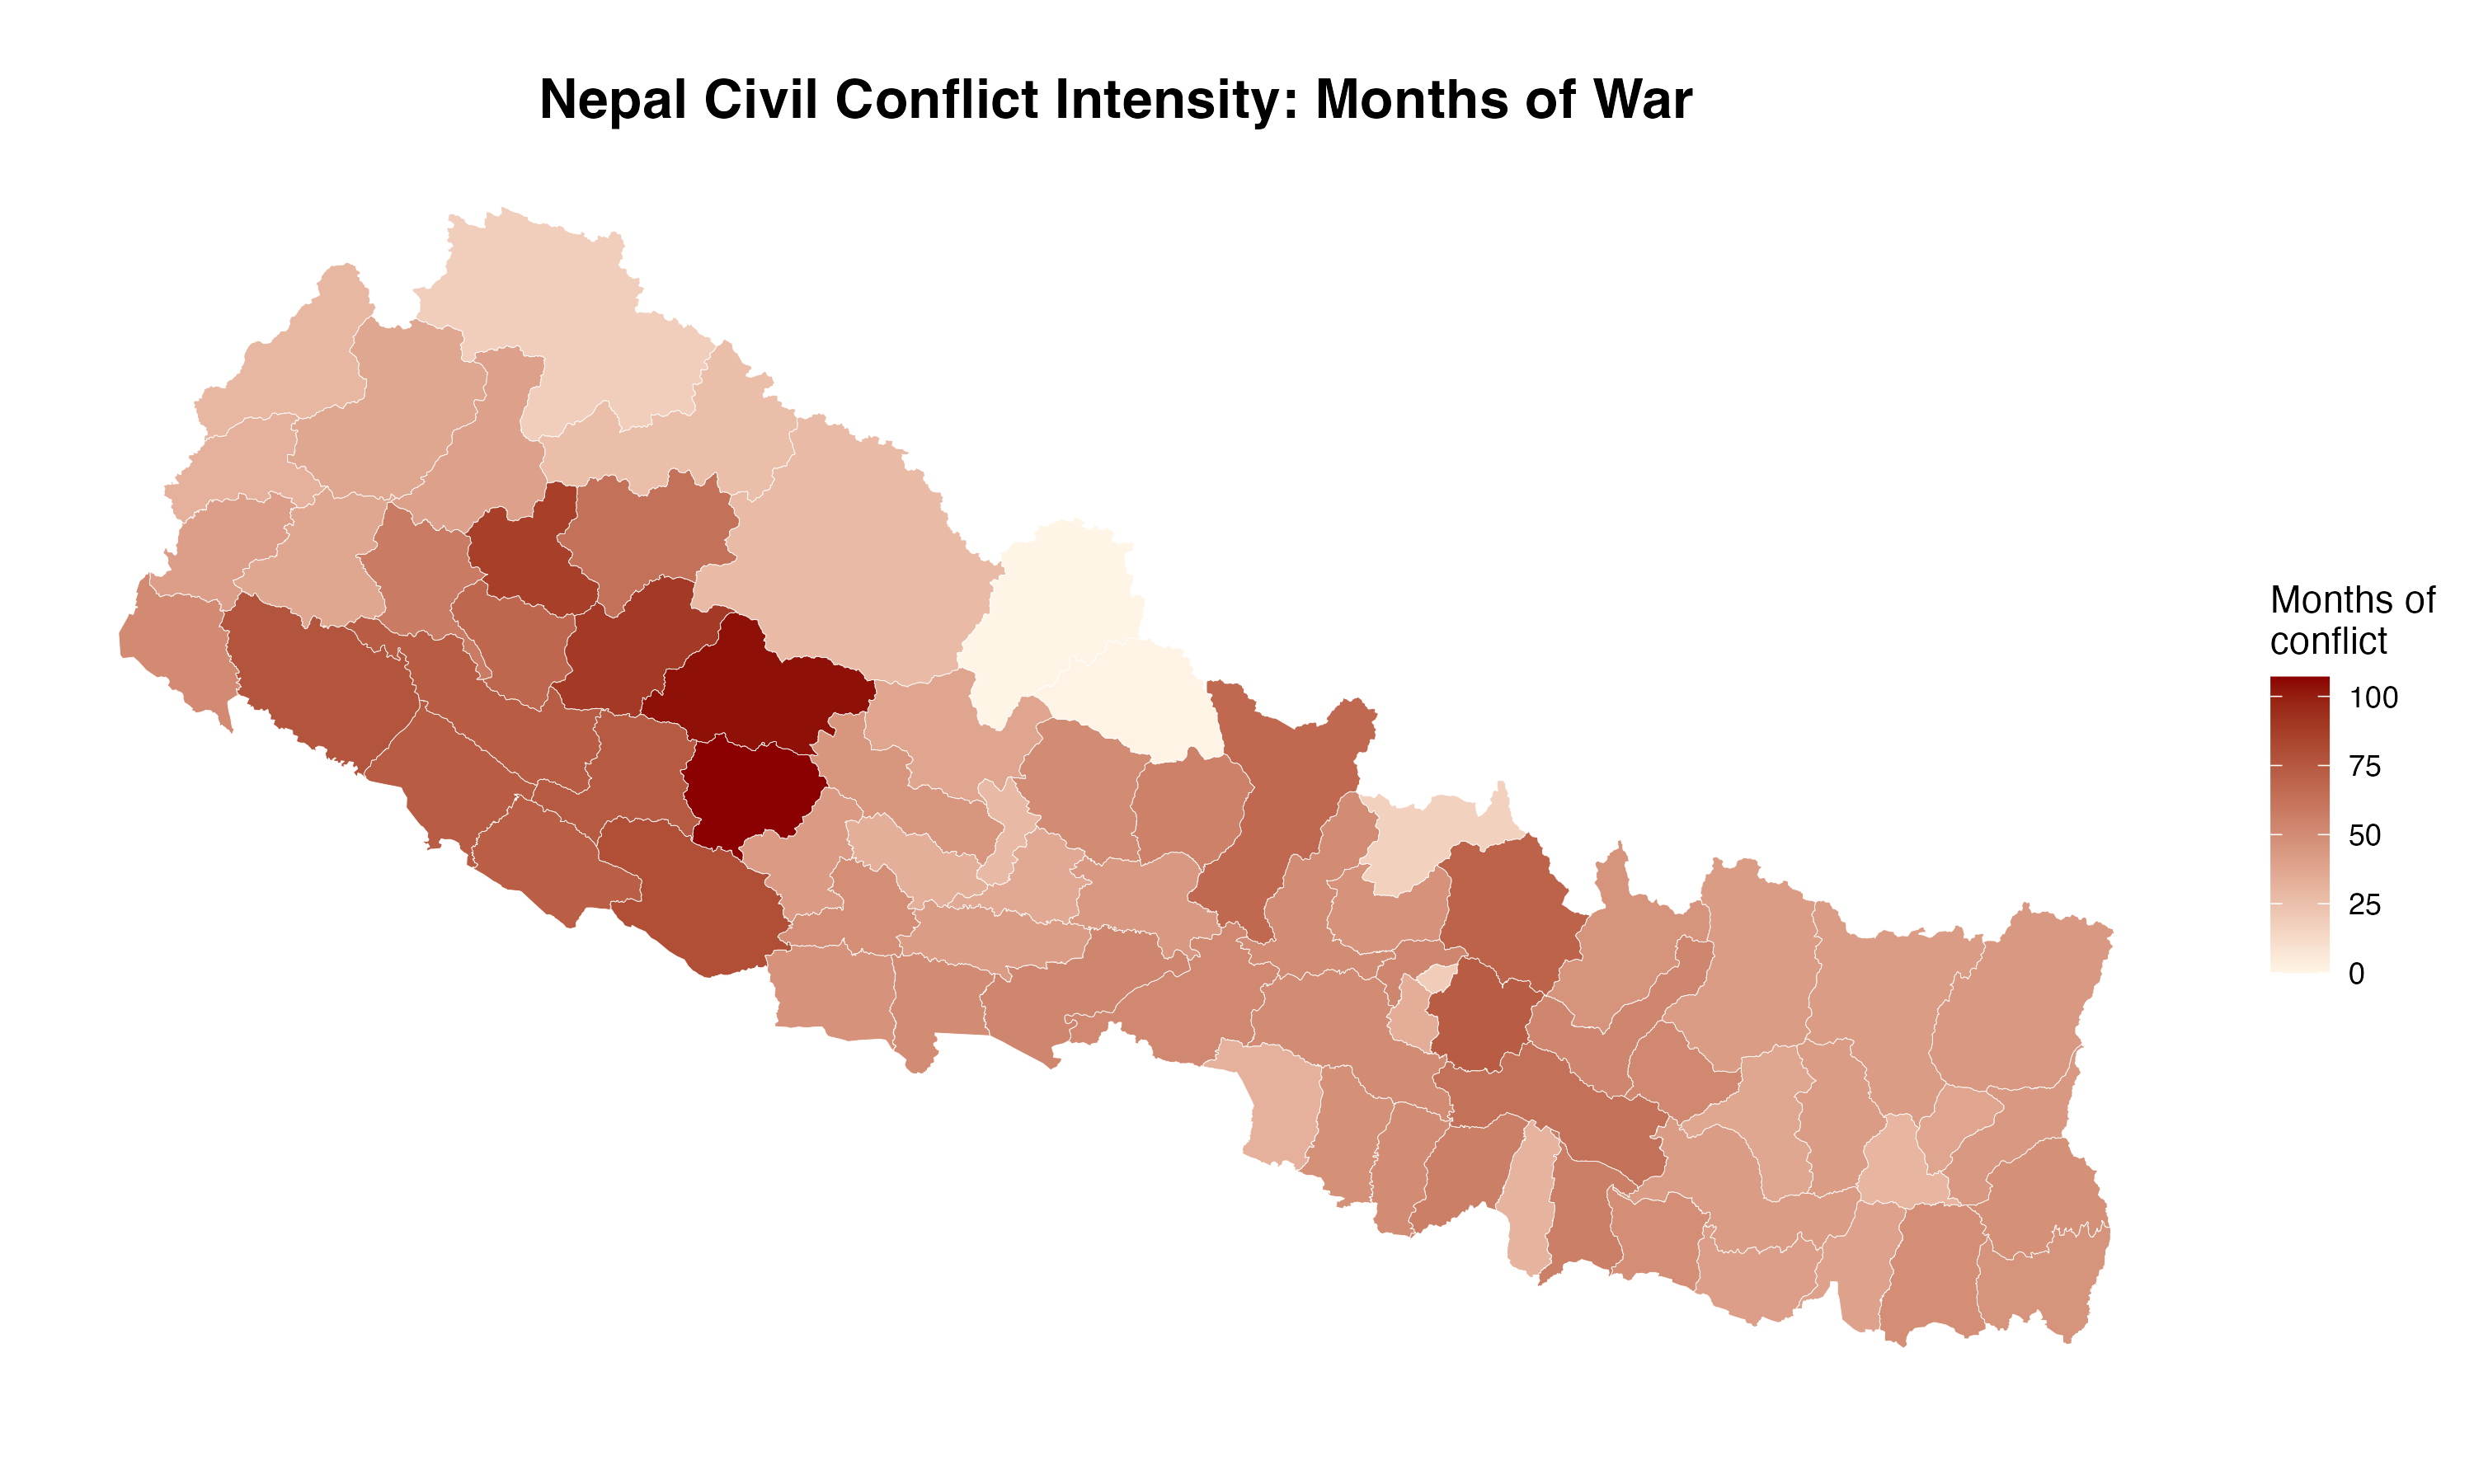
\includegraphics[width=0.85\textwidth]{Paper/Figures/month_of_war_intensity_1.png}
    \caption{High-Conflict Districts (Months of War, $75^{th}$ Percentile Cutoff)}
    \label{fig:conflict_map}
    \begin{minipage}{0.9\textwidth}
        \footnotesize
        \emph{Notes:} Districts shaded in dark are classified as high-conflict 
        ($P_d = 1$); districts in light shading are low-conflict ($P_d = 0$). 
        Classification is based on whether the total months of war (Equation~\ref{eq:months_of_war}) 
        exceeds the 75th percentile across all districts. Source: Authors' 
        calculations from INSEC conflict database (1996--2006). Alternative 
        intensity measures and continuous versions are reported in Appendix. 
        \end{minipage}
\end{figure}

We report results using the casualty-based binary measure as a robustness 
check and the continuous versions of both measures in Appendix~\ref{appendix:robustness}.



\subsection{Descriptive Statistics}


\begin{table}[H]
\centering
\caption{\label{tab:tab:overall_summary}Descriptive Statistics: Overall Sample}
\centering
\fontsize{10}{12}\selectfont
\begin{threeparttable}
\begin{tabular}[t]{lrrr}
\toprule
Variable & Mean / \% & SD & N\\
\midrule
Panel A: Migration outcomes &  &  \vphantom{4} & \\
International Migrant (=1) & 10.85 & 31.11 & 90,109\\
Currently Abroad (=1) & 8.29 & 27.57 & 90,074\\
Return Migrant (=1) & 3.01 & 17.09 & 77,638\\
Internal Migrant (=1) & 5.52 & 22.83 & 90,050\\
\addlinespace
Absent from Household (=1) & 13.84 & 34.53 & 90,109\\
 &  &  \vphantom{3} & \\
Panel B: Exposure to conflict (1996-2006) &  &  \vphantom{2} & \\
Months of War (any) & 53.57 & 17.00 & 90,109\\
Months of War (fatal) & 49.91 & 16.76 & 90,109\\
\addlinespace
Casualties (any) & 244.64 & 175.66 & 90,109\\
Casualties (fatal) & 213.58 & 159.08 & 90,109\\
 &  &  \vphantom{1} & \\
\textbf{Panel C: Demographics} & \textbf{} & \textbf{} & \textbf{}\\
Age in 2017 & 27.70 & 19.43 & 90,109\\
\addlinespace
Age at Conflict Start (1996) & 6.70 & 19.43 & 90,109\\
Male (=1) & 51.24 & 49.98 & 90,109\\
Marital Status (\%): &  &  & \\
    Divorced & 0.07 &  & 45\\
    Married & 62.13 &  & 38,345\\
\addlinespace
    Never Married & 32.21 &  & 19,878\\
    Separated & 0.40 &  & 248\\
    Single & 5.19 &  & 3,201\\
 &  &  & \\
\textbf{Panel D: Education} & \textbf{} & \textbf{} & \textbf{}\\
\addlinespace
Years of Education & 7.43 & 4.03 & 61,951\\
 Education Distribution (\%): &  &  & \\
    No Education & 2.67 &  & 1,654\\
    Primary (1-5) & 35.81 &  & 22,183\\
    Secondary (6-12) & 56.70 &  & 35,129\\
\addlinespace
    Tertiary & 4.82 &  & 2,985\\
 &  &  & \\
\textbf{Panel E: Ethnicity (\%)} & \textbf{} & \textbf{} & \textbf{}\\
    Dalit & 14.48 &  & 13,024\\
    Hill High Caste & 36.92 &  & 33,214\\
\addlinespace
    Hill Janajati & 27.44 &  & 24,690\\
    Muslim & 3.44 &  & 3,098\\
    Terai/Madhesi & 17.72 &  & 15,937\\
 &  &  & \\
\textbf{Panel F: Occupation (\%)} & \textbf{} & \textbf{} & \textbf{}\\
\addlinespace
    Agriculture & 10.25 &  & 2,542\\
    Armed Forces & 1.79 &  & 445\\
    Craft \& Manufacturing & 23.85 &  & 5,918\\
    Elementary/Low Skilled & 24.72 &  & 6,132\\
    High Skilled & 10.39 &  & 2,577\\
\addlinespace
    Service \& Clerical & 29.00 &  & 7,196\\
\bottomrule
\end{tabular}
\begin{tablenotes}
\item \textit{Notes:} 
\item International Migrant includes individuals abroad at time of survey and those who had been abroad for at least 3 months in the past.
\item Currently Abroad includes individuals abroad at the time of survey.
\item Return Migrant includes only individuals who travelled abroad for at least 3 months.
\item Internal Migrant includes individuals migrating inside the country at the time of survey.
\item Absent from Household includes all absent individuals at the time of survey.
\item Distribution percentages within Panels C-F are computed on non-missing observations. Missing counts: Education = 28,158; Ethnicity = 146; Marital Status = 28,392; Occupation = 65,299.
\item Occupation percentages exclude 2,334 observations coded 'Not Stated' (NSCO code 9999) and 1,726 absent household members whose occupation was not reported by the household respondent.
\item Source: Nepal Labour Force Survey 2017/18; conflict exposure data from INSEC (1996-2006).
\end{tablenotes}
\end{threeparttable}
\end{table}


\newpage
\input{Paper/Tables/Tables_Summary/7.Multigroup_Summary}


% \newpage
% \input{Summary Tables/Summary Stat by Treatment }

% %\newpage
% %\begin{table}[!h]
\centering
\caption{\label{tab:tab:cohort_summary}Summary Statistics by Cohort}
\centering
\resizebox{\ifdim\width>\linewidth\linewidth\else\width\fi}{!}{
\fontsize{9}{11}\selectfont
\begin{tabular}[t]{lrrrrr}
\toprule
Variable & T1 (0-3) & T2 (4-8) & T3 (9-15) & C1 (16-21) & C2 (22-29)\\
\midrule
N & 9319 & 7985 & 8040 & 6760 & 6292\\
Absent (\%) & 22.44 & 24.58 & 23.81 & 10.84 & 16.18\\
 &  &  &  &  & \\
Months of War & 53.58 & 53.32 & 53.48 & 52.94 & 53.36\\
 & (16.92) & (16.7) & (16.66) & (16.34) & (16.7)\\
\addlinespace
Casualties & 244.7 & 245 & 245.09 & 240.29 & 243.95\\
 & (176.12) & (176.2) & (175.79) & (173.13) & (175.01)\\
Age in 2017 & 32.99 & 26.88 & 22.48 & 46.42 & 39.54\\
 & (2.06) & (1.39) & (1.12) & (2.24) & (1.68)\\
Age at Conflict Start & 11.99 & 5.88 & 1.48 & 25.42 & 18.54\\
\addlinespace
 & (2.06) & (1.39) & (1.12) & (2.24) & (1.68)\\
Male (\%) & 50.58 & 51.8 & 52.41 & 50.47 & 49.83\\
Education Distribution &  &  &  &  & \\
No Education (\%) & 4.23 & 1.92 & 1.18 & 8.65 & 5.69\\
Primary (\%) & 27 & 19.66 & 13.12 & 34.36 & 31.03\\
\addlinespace
Secondary (\%) & 59.62 & 66.03 & 77.78 & 49.94 & 55.63\\
Tertiary (\%) & 9.15 & 12.39 & 7.93 & 7.04 & 7.65\\
Ethnic Distribution &  &  &  &  & \\
Hill High Caste (\%) & 36.89 & 35.23 & 34.07 & 37.58 & 36.51\\
Hill Janajati (\%) & 26.86 & 27.42 & 28.44 & 28.77 & 28.51\\
\addlinespace
Terai/Madhesi (\%) & 20.01 & 20.63 & 20.19 & 18.98 & 19.75\\
Dalit (\%) & 13.31 & 13.58 & 14.02 & 11.85 & 12.37\\
Muslim (\%) & 2.93 & 3.14 & 3.27 & 2.82 & 2.86\\
\bottomrule
\end{tabular}}
\end{table}

% \newpage
% \input{Summary Tables/Summary Stat by Cohort}

% \newpage
% \input{Summary Tables/Summary by Conflict Intensity}

% % %\newpage
% % %\begin{table}[!h]
\centering
\caption{\label{tab:balance_check}Balance Check: Treatment vs Control Groups}
\resizebox{0.8\textwidth}{!}{%
\begin{threeparttable}
\begin{tabular}{lrrrr}
\toprule
Variable & Control & Treatment & Difference & P-Value \\
\midrule
\textbf{Outcome:} & & & & \\
Absent (\%) & 13.42 & 23.55 & 13.5 & 0*** \\
 & (0.3) & (0.27) & & \\
 & & & & \\
\textbf{Conflict Exposure:} & & & & \\
Months of War & 53.14 & 53.47 & 0.32 & 0.069295* \\
 & (0.14) & (0.11) & & \\
Casualties & 242.05 & 244.92 & 2.87 & 0.128043 \\
 & (1.52) & (1.11) & & \\
 & & & & \\
\textbf{Demographics:} & & & & \\
Age in 2017 & 43.1 & 27.73 & -15.37 & 0*** \\
 & (0.03) & (0.03) & & \\
Age at Conflict Start & 22.1 & 6.73 & -15.37 & 0*** \\
 & (0.03) & (0.03) & & \\
Male (\%) & 50.16 & 51.55 & 1.4 & 0.010089** \\
 & (0.44) & (0.31) & & \\
 & & & & \\
\textbf{Education:} & & & & \\
No Education (\%) & 7.07 & 2.43 & -4.6 & 0*** \\
 & (0.22) & (0.1) & & \\
Primary (\%) & 32.58 & 19.83 & -12.7 & 0*** \\
 & (0.41) & (0.25) & & \\
Secondary (\%) & 52.99 & 67.96 & 15 & 0*** \\
 & (0.44) & (0.29) & & \\
Tertiary (\%) & 7.37 & 9.77 & 2.4 & 0*** \\
 & (0.23) & (0.19) & & \\
 & & & & \\
\textbf{Ethnicity:} & & & & \\
Hill High Caste (\%) & 37.08 & 35.53 & -1.6 & 0.00643*** \\
 & (0.42) & (0.3) & & \\
Hill Janajati (\%) & 28.65 & 27.51 & -1.1 & 0.031793** \\
 & (0.4) & (0.28) & & \\
Dalit (\%) & 12.09 & 13.61 & 1.5 & 0.000113*** \\
 & (0.29) & (0.22) & & \\
\bottomrule
\end{tabular}
\begin{tablenotes}
\footnotesize
\item \textit{Notes:} Standard errors in parentheses. *** $p<0.01$, ** $p<0.05$, * $p<0.10$. T-tests for difference in means between treatment and control groups.
\end{tablenotes}
\end{threeparttable}
}
\end{table}




% % \newpage
% % % \input{Summary Tables/T-test of Differenct}

% % %\newpage
% % %\begin{table}[!h]
\centering
\caption{\label{tab:tab:did_framework}Absenteeism Rates by Treatment Status and Conflict Intensity }
\centering
\fontsize{10}{12}\selectfont
\begin{tabular}[t]{llrrr}
\toprule
Group &  & No Conflict & Low Conflict & High Conflict\\
\midrule
\addlinespace[0.3em]
\multicolumn{5}{l}{\textbf{Control Cohort }}\\
\hspace{1em} & Absent (\%) & 0 & 13.5 & 13.33\\
\hspace{1em} & N & 7 & 7395 & 5650\\
\addlinespace[0.3em]
\multicolumn{5}{l}{\textbf{Treatment Cohort }}\\
\hspace{1em} & Absent (\%) & 9.38 & 24.94 & 21.84\\
\hspace{1em} & N & 32 & 14107 & 11205\\
\bottomrule
\end{tabular}
\end{table}
% % %\vspace{3cm}
% % %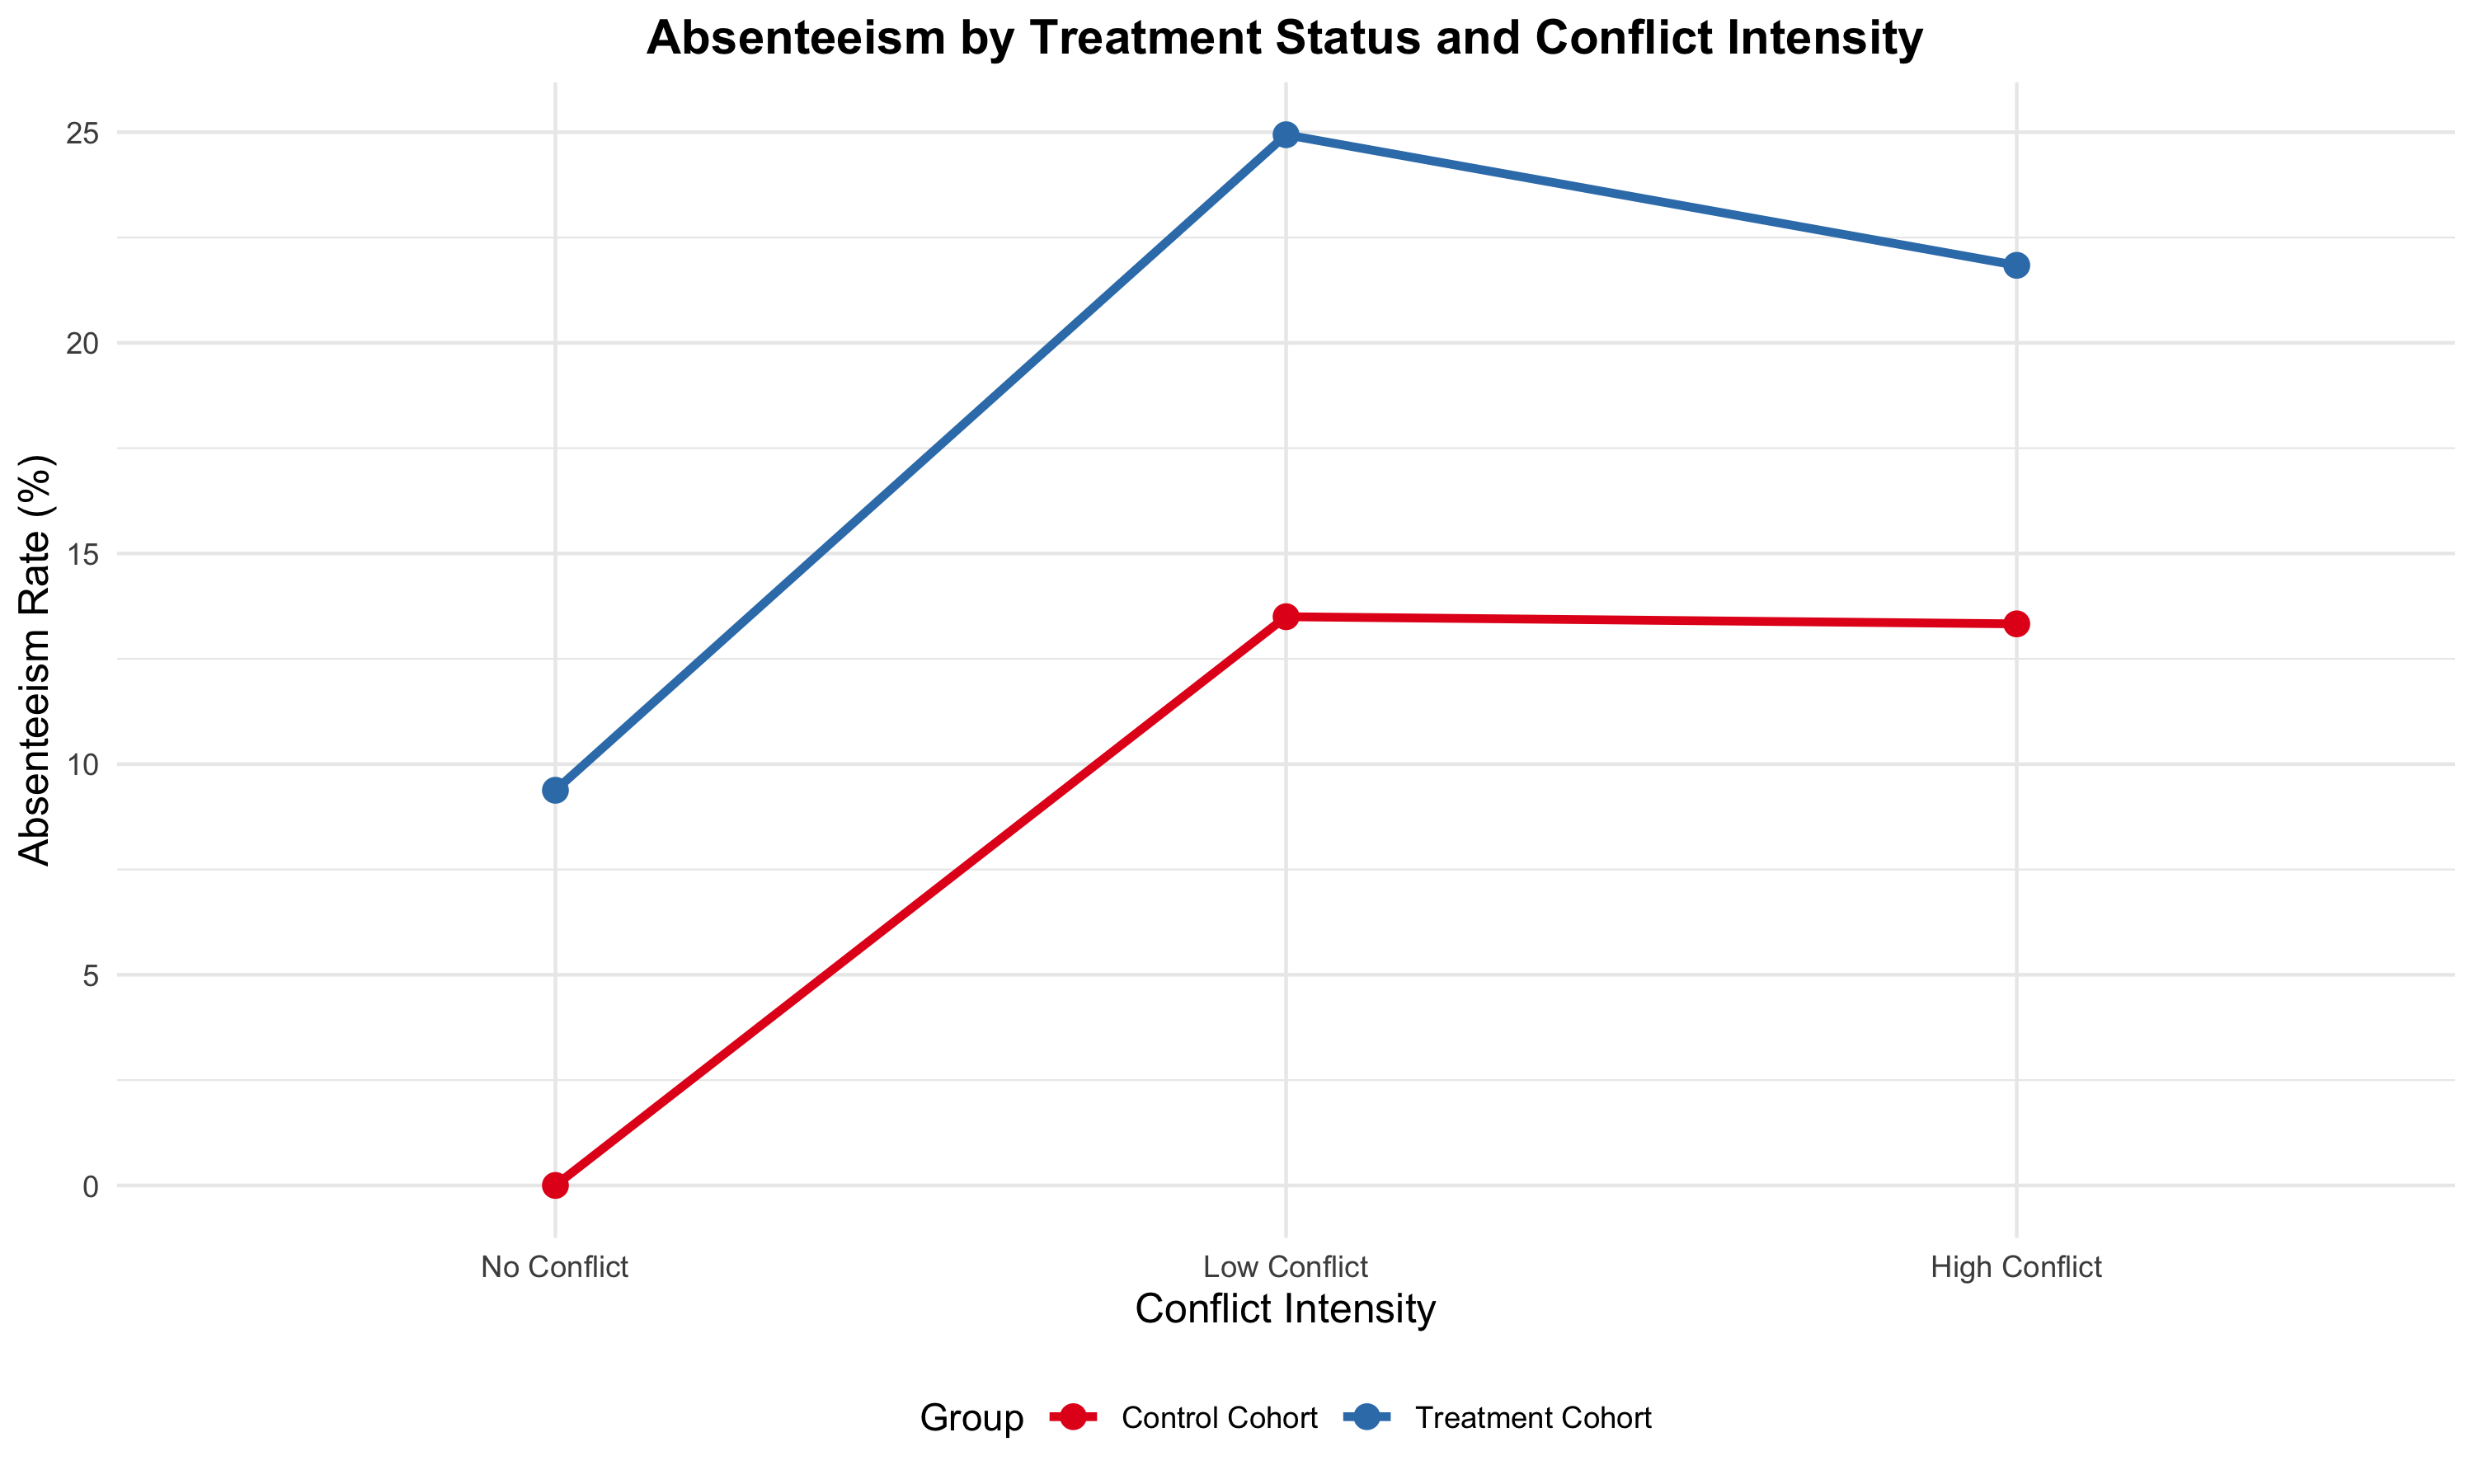
\includegraphics[width=0.8\textwidth]{figures/Figure1_DID_Framework.png}

% % \newpage
% % \begin{table}[!h]
\centering
\caption{\label{tab:tab:did_war}DID Framework: International Migration by Treatment Status and Conflict Intensity (War-Based)(New)}
\centering
\fontsize{10}{12}\selectfont
\begin{tabular}[t]{lrrr}
\toprule
 & Low Conflict & High Conflict & Difference (H - L)\\
\midrule
Control Cohort & 5.13\% & 8.29\% & 3.16 \\
 & (n=7680) & (n=2050) & \\
Treatment Cohort & 23.45\% & 21.81\% & -1.64 \\
 & (n=21095) & (n=6349) & \\
Difference (T - C) & 18.32  & 13.52  & DID: -4.8 \\
\addlinespace
 &  &  & \\
\bottomrule
\end{tabular}
\end{table}
% % \vspace{3cm}
% % \begin{table}[!h]
\centering
\caption{\label{tab:tab:did_casualty}DID Framework: International Migration by Treatment Status and Conflict Intensity (Casualty-Based)(New)}
\centering
\fontsize{10}{12}\selectfont
\begin{tabular}[t]{lrrr}
\toprule
 & Low Conflict & High Conflict & Difference (H - L)\\
\midrule
Control Cohort & 4.71\% & 9.76\% & 5.05 \\
 & (n=7639) & (n=2091) & \\
Treatment Cohort & 23.31\% & 22.3\% & -1.01 \\
 & (n=20907) & (n=6537) & \\
Difference (T - C) & 18.6  & 12.54  & DID: -6.06 \\
\addlinespace
 &  &  & \\
\bottomrule
\end{tabular}
\end{table}


